% Nome do capítulo
\chapter{Results}
% Label para referenciar
\label{cap5}

% Diminuir espaçamento entre título e texto
\vspace{-1.9cm}

% Texto do capítulo

In this Chapter, we use Belo Horizonte as a study case to validate \textit{PondiônsTracker} using
\textit{PondiônsTracker-BH}. We used the GTFS file published on July 23${^{th}}$ 2023 and collected
data from the real-time API for eleven days straight, from 29-07-2023 to 08-08-2023.
During this period, our script was executed every minute, summarizing over 246 million entries 
representing almost 30 Gigabytes, Table \ref{tab:entries} presents the entries for each day collected.

\begin{table}[h]
\centering
\caption{Workload Overview } 
\begin{tabular}{ |c|c|c|l| } 
\hline
Date & Day-of-Week & Entries \\
\hline
29-07-23& Saturday & 22,319,765 \\ 
\hline
30-07-23& Sunday & 22,635,117 \\ 
\hline
31-07-23& Monday & 22,583,380 \\ 
\hline
01-08-23& Tuesday & 22,432,739 \\ 
\hline
02-08-23& Wednesday & 21,970,073 \\ 
\hline
03-08-23& Thursday & 22,050,579 \\ 
\hline
04-08-23& Friday & 22,402,865 \\ 
\hline
05-08-23& Saturday & 22,642,955 \\ 
\hline
06-08-23& Sunday & 22,786,254 \\ 
\hline
07-08-23& Monday & 22,109,606 \\ 
\hline
08-08-23& Tuesday & 22,405,222 \\ 
\hline
\textbf{Total}& - & \textbf{246,338,555} \\ 
\hline
\end{tabular}
\source{The authors}
\label{tab:entries}
\end{table}


We also present an analysis of the data collected, which is based on the output of 
\textit{PondiônsTracker-BH}'s \textit{IntegrationDriver} for {\em all} routes scheduled in
the GTFS during the observation period. Firstly, we compare the expected with the real scenarios of Belo Horizonte's PTN over the observed period, and then we deepen into out-of-schedule incidents, especially delays. The following analysis are divided into three groups: Weekdays, Saturday and Sunday. This happens due to the GTFS $service\_id$ field, as previously discussed in Chapter 2.


\section{Schedule Analysis}

Table \ref{tab:schedule}
shows that every observed day have $294$ \textit{Routes} planned. For weekdays are planned $22,774$ \textit{Trips},
$14,100$ for Saturdays and $9,133$ for Sundays. Table \ref{tab:schedule} shows the schedule-filled percentage of trips filled with real-time trips during the observation period. This translates to the percentage of trips planned by the trips collected and matched from the real-time API.

\begin{table}[h]
\centering
\caption{Belo Horizonte's PTN} 
\begin{tabular}{|c|c|r|r|c|}
\hline
Date & Routes    & Scheduled Trips  & Matched Trips & $\%$ \\ \hline
29-07-23 & 294 &  14,100 &     11,424   & 81.02\%\\ \hline
30-07-23 & 294 & 9,133 &  7,594  &   83.14\% \\ \hline
31-07-23 & 294 & 22,774 &  17,184  &   75.45\%  \\ \hline
01-08-23 & 294 & 22,774 &  16,948  &   74.42\%  \\ \hline
02-08-23 & 294 & 22,774 &  16,914  &   74.27\%  \\ \hline
03-08-23 & 294 & 22,774 & 16,973  &   74.53\%  \\ \hline
04-08-23 & 294 & 22,774 &  16,854  &   74.01\%  \\ \hline
05-08-23 & 294 & 14,100 &  11,372  &   80.65\%  \\ \hline
06-08-23 & 294 & 9,133 &  7,679  &   84.08\%  \\ \hline
07-08-23 & 294 & 22,774 & 16,849  &   73.98\%  \\ \hline
08-08-23 & 294 & 22,774 &  16,837  &   73.93\%  \\ \hline
\textbf{Total} & \textbf{3,234} & \textbf{205,884} &  \textbf{156,628}  &   \textbf{$76.08\%$}  \\ \hline
\end{tabular}
\source{The authors}
\label{tab:schedule}
\end{table}

\begin{figure}[h!]
     \centering
        \caption{Histograms Schedule-Filled Percentage per Routes}
        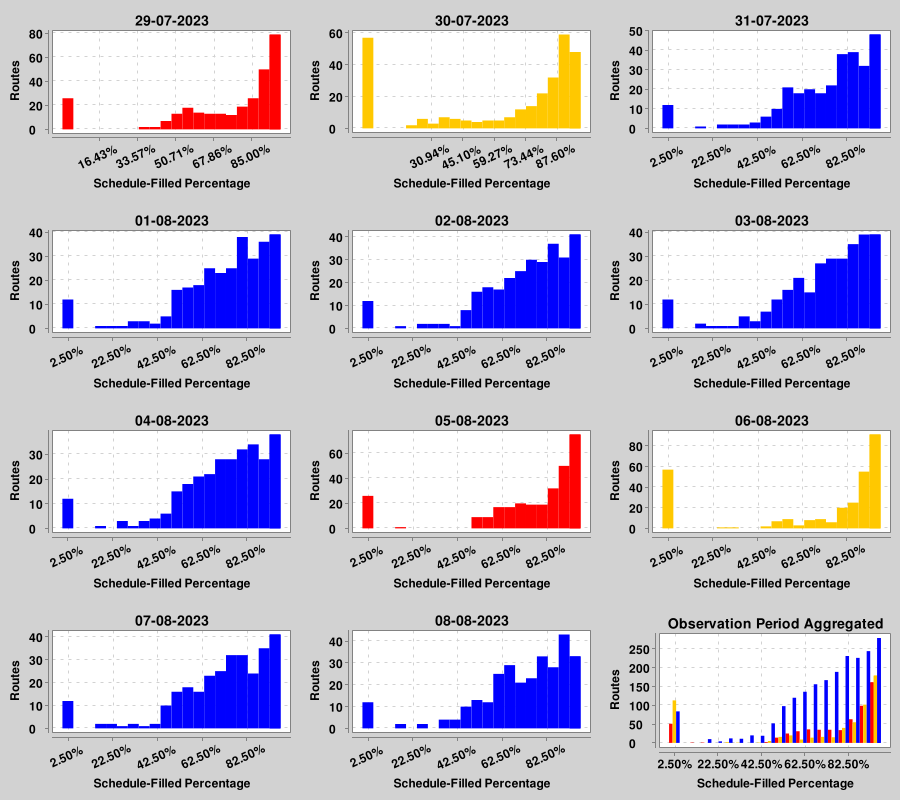
\includegraphics[width=\textwidth]{imagem/cap5/histogram_schedule-Filled.png}
        %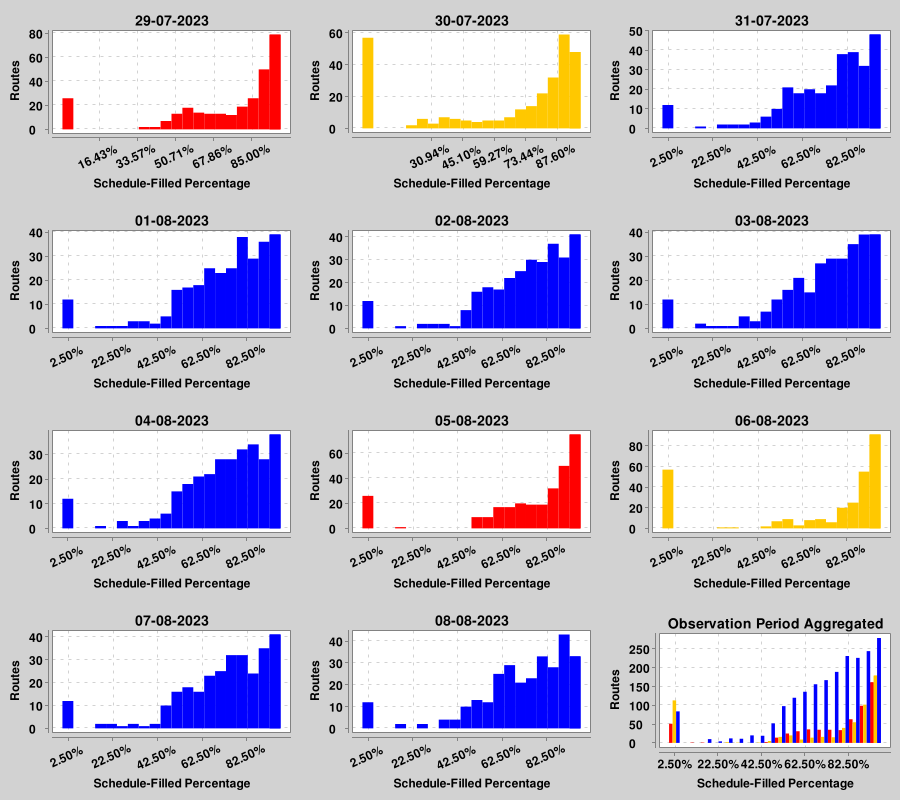
\includegraphics[scale=.3]{imagem/cap5/histogram_schedule-Filled.png}
        \source{The authors}
        \label{img:5:hist}
\end{figure}

The schedule-filled percentage values correspond to {\em all} the $3,234$ routes scheduled, and it has an average for all the period of
$76.08\%$, but this ratio is{ \em indirectly proportional} to the number of scheduled trips. 
Weekdays have the biggest number of $159,418$ trips defined and the lowest average for matched trips of
$74,37\%$, comprised by 31-07, 01-08, 02-08, 03-08, 04-08, 07-08 and 08-08.
Saturday's average is $80.84\%$ with $28,200$ scheduled trips, comprised of days 29-07 and 05-08.
Finally, Sunday's average is $83.61\%$ with $18,266$ scheduled trips comprised of days 30-07 and 06-08.

Figure \ref{img:5:hist} shows the histograms of the schedule-filled percentage distributed throughout each day, and
the last histogram presents the aggregated distribution for the observation period. The red, yellow, and blue bars represent Saturday, Sunday, and Weekdays. All histograms present that the schedule is not uniformly distributed,
and despite the averages shown in Table \ref{tab:schedule}, for each day, the most considerable individual 
frequencies are associated with the schedule-filled percentage of at least $82.50\%$, as shown in the aggregated histogram. 

All histograms show the existence of considerable sets of routes whose schedule-filled percentage is {\em at most} $42.50$\%, and, especially, routes with near 0 routes reported. These sets are 
likely caused by the unpredictable and randomness of the network, leading to unwanted and unfinished trips, as discussed in the previous Chapter. Which decreases the averages and points to a high standard deviation, representing that the schedule is not uniformly distributed. Then, plenty of routes are completed ($100\%$) or at least near $82.50\%$, despite some associated with lower percentages.


Regarding the real-time API, there are $4,095$ collected trips from $63$ different routes which were not defined at Belo 
Horizonte's GTFS. In other words, the API provided $4,095$ trips with a valid $NV$ unscheduled 
trips. Table \ref{tab:unscheduledTrips} shows the top 5 routes with the most unscheduled trips. 
For instance, the route $82$ has a high schedule-filled rate  with real-time trips despite having the most
unscheduled trips. On Sundays, the GTFS does not schedule any trip for route $82$,
but the API provided 
entries regarding this route twice during the period observed.
The first time with $147,897$ entries leading to $505$ trips collected 
and the second time with $149,422$ entries leading to $551$ trips collected , then once added gets to the $1,056$ shown in Table \ref{tab:unscheduledTrips}.

\begin{table}[h]
\centering
\caption{Top 5 Routes With The Most Unscheduled Trips} 
\begin{tabular}{|l|c|}
\hline
Route & Unscheduled Trips  \\ \hline
\textit{82 - Estação São Gabriel / Savassi Via Hospitais} & 1,056 \\ \hline
\textit{61 - Estação Venda Nova/Centro-Direta} & 791 \\ \hline
\textit{52 - Estação Pampulha / Avenida Antonio Carlos} & 612 \\ \hline
\textit{50 - Estação Pampulha / Centro - Direta} & 309 \\ \hline
\textit{85 - Estação São Gabriel / Centro Via Floresta} & 257 \\ \hline
\end{tabular}
\source{The authors}
\label{tab:unscheduledTrips}
\end{table}



\section{Delay Analysis}
To analyze the delays in the PTN, firstly, we take a look at the delays on a global scale of the network, and for the context of this section, to be {\em on-time} denotes that the expected time is equal to the real-time
within a maximum fifty-nine-seconds span, so a {\em delay} is a time after the expected and a {\em ahead-of-schedule}
is a time before the expected, with equal or greater than one minute.
In this context, Table \ref{tab:delay1} presents data over the matched trips aggregated by the day of the week, 
in which the trips entirely out of schedule represent the most extensive set of trips. The definition of this group is that every trip 
does not have a single entry on time. In other words, for these trips, the buses were either delayed
or ahead of schedule for all expected times at every bus stop. 



\begin{table}[h]
\centering
\caption{Delays detailed in whole PTN scale } 
\begin{tabular}{|l|r|r|r|}
\hline
\multicolumn{1}{|c|}{} & Weekday    & Saturday    & Sunday  \\ \hline
Total trips  matched & 118,559 &  22,796  & 15,273\\ \hline
Trips entirely out of schedule & 60,244  & 10,899 & 7,148\\ \hline
Trips with departure or arrival on time & 39,403 & 8,731 &    5,988\\ \hline
Trips with departure and arrival on time & 324 & 95 & 56 \\ \hline
Trips entirely on time & 1 & 2 &  1\\ \hline
\end{tabular}
\source{The authors}
\label{tab:delay1}
\end{table}

Furthermore, Table's \ref{tab:delay1} second and third
most extensive sets are related to trips that are on-time at the beginning and the end of the trip. The
third group represents if the trip is on time on both ends, and it is contained by the second group, which requires
at least one end on time. The second group also contains the last group, a particular case of the bus being on time for {\em all} bus stops in the trip, which occurred only four times during the observation period for the same route, coincidentally.
The route is \textit{331 - Estação Barreiro/Conjunto Antonio Teixeira Dias Via Upa}, which has 32 bus stops, representing a length of 8,948.92 meters, almost 9 kilometers, and the four expected and real date-times are listed as follows:
\begin{enumerate}
    \item Expected departure and arrival: Jul. 29 15:30:00 - 15:56:27 \\ Real departure and arrival: Jul. 29 15:30:03 - 15:57:03;
    \item Expected departure and arrival: Jul. 30 08:20:00 - 08:46:27 \\ Real departure and arrival: Jul. 30 08:20:31 - 08:46:15;
    \item Expected departure and arrival: Aug. 04 05:40:00 - 06:06:27 \\ Real departure and arrival: Aug. 04 05:40:30 - 06:06:00;
    \item Expected departure and arrival: Aug. 05 17:10:00 - 17:36:27 \\ Real departure and arrival: Aug. 05 17:10:45 - 17:36:49.
\end{enumerate}

\begin{figure}[h!]
     \centering
        \caption{$DELAY$s Distribution: Bus Stop and Trip}
        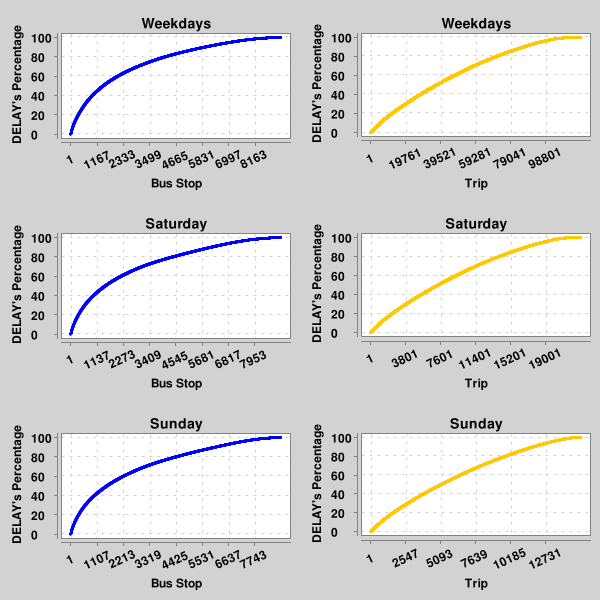
\includegraphics[scale=.45]{imagem/cap5/trips_delays_per_bus_stops.png}
       % 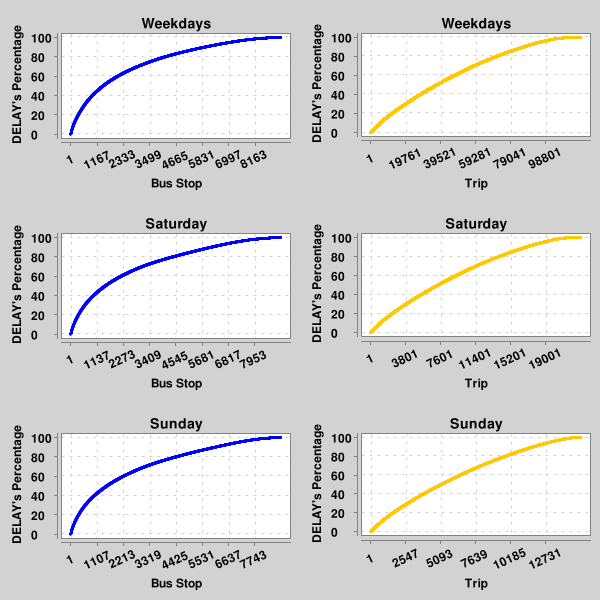
\includegraphics[width=\textwidth]{imagem/cap5/trips_delays_per_bus_stops.png}
        \source{The authors}
        \label{img:5:DelayDistribution}
\end{figure}

Until this point, our analysis has not taken into account the impact of each distinct status in the PTN, and for weekdays, the statuses are divided as:
\begin{enumerate*}
    \item DELAY representing $89.8\%$;
    \item AHEAD\_OF\_SCHEDULE representing $6.9\%$;
    \item ON\_TIME representing $3.3\%$.
\end{enumerate*}
The predominance of $DELAYED$ in the PTN does not imply that the network is not working 
nor completely stopped because the $DELAYED$s are {\em log-normal} distributed between the bus stops and trips, as shown in Figure \ref{img:5:DelayDistribution}.
So, this leads to the scenario where few bus stops and trips cause more delays. 
For instance, for all delays reported for weekdays, 200 trips represent $14.05\%$, and 200 bus stops $73.75\%$. This distribution also occurs on Saturdays and Sundays, as shown in Figure \ref{img:5:DelayDistribution}.



The distribution indicates a small set of bus stops is responsible for most delays, but it does not imply any spatial relationships between this set. Figure \ref{img:5:mostDelayedStops} shows $2,115$ out of $9,309$ most delayed bus stops, representing around $60\%$ of the total delay and only $22.72\%$ of the bus stops. It is observable that some main avenues
and pathways are contemplated, such as the following:
\begin{enumerate*}
    \item \textit{Avenida Dom Pedro II};
    \item \textit{Rua Padre Eustáquio};
    \item \textit{Avenida Amazonas}.
\end{enumerate*}

\begin{figure}[h]
\centering
\begin{minipage}[t]{.5\textwidth}
  \centering
  \caption{300 Most Delayed Stops}
  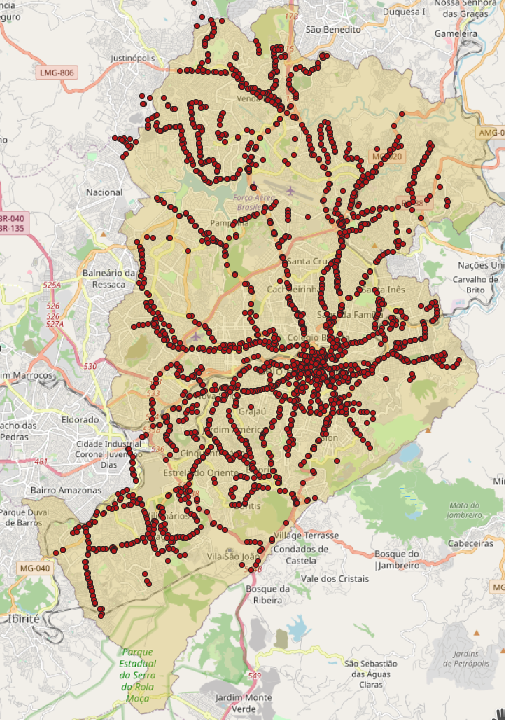
\includegraphics[width=.90\linewidth]{imagem/cap5/mostDelayedStops.png}
  \source{The authors}
  \label{img:5:mostDelayedStops}
\end{minipage}%
\begin{minipage}[t]{.5\textwidth}
  \centering
  \caption{Fragment of the 50 Most \\Delayed Stops }
  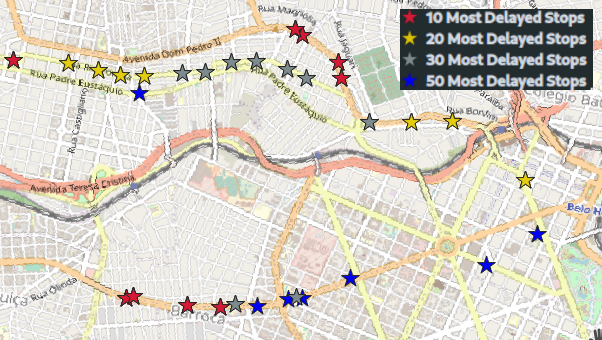
\includegraphics[width=\linewidth]{imagem/cap5/10-50MostDelayedStops.png}
  \source{The authors}
  \label{fig:50mostDelayedStops}
\end{minipage}
\end{figure}

These three pathways are represented in Figure \ref{fig:50mostDelayedStops}, which shows a 
fragment of Belo Horizonte's PTN and indicates the 50 most delayed stops divided into groups
regarding the number of delays. So, the stops in red accumulate the most delays, and
the group in blue gathers the fewest for this figure, yet these stops represent $4.58$\% of the network.
Also, Figure \ref{fig:50mostDelayedStops} reveals the spatial relationships between these stops
because they are on the same pathway. For instance, the \textit{Avenida Amazonas}, the avenue located in the lower part of the figure, is one of the most critical avenues in the PTN, containing dozens of stops throughout its 8.97 kilometers, \textit{Avenida Amazonas} has 10 out of the 50 most delayed
stops. As follows, we list the 5 most delayed stops for weekdays during the observation period:

\begin{enumerate}
    \item $\#14793268$ - \textit{Avenida Dom Pedro II 1520} with $7,309$ delays reported at;
    \item $\#14791617$ - \textit{Avenida Amazonas 7309} with $7,009$ delays reported at;
    \item $\#14790997$ - \textit{Avenida Dom Pedro II 1980} with $6,692$ delays reported at;
    \item $\#14784438$ - \textit{Avenida Sinfronio Brochado 773} with $6,528$ delays reported at;
    \item $\#14788981$ - \textit{Avenida Amazonas 3410} with $6,272$ delays reported at.
\end{enumerate}


\begin{figure}[b]
     \centering
        \caption{Minutes out of schedule of bus stops $\#14788408$ distributed throughout the day}
        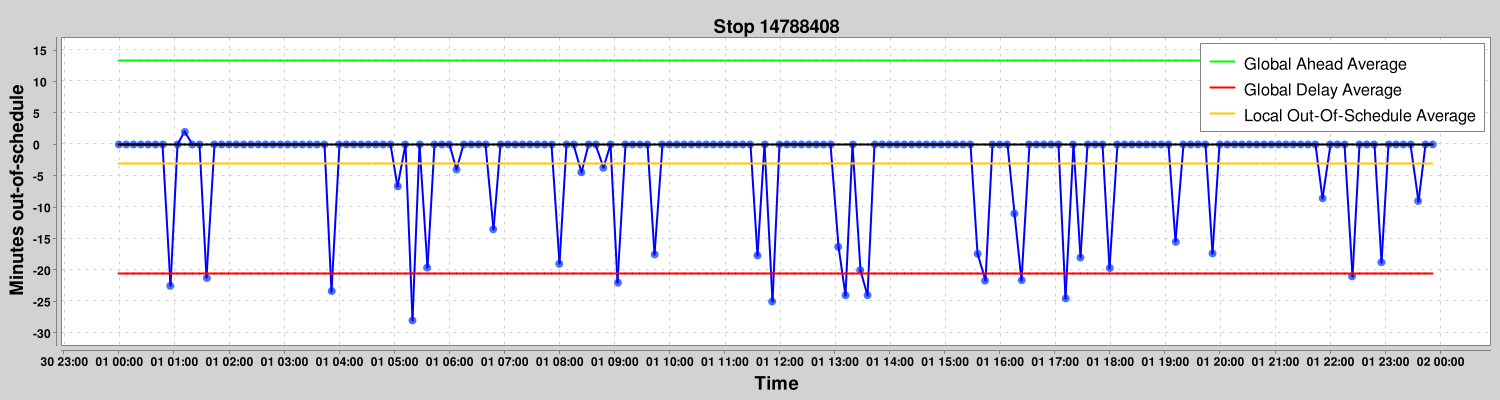
\includegraphics[width=\textwidth]{imagem/cap5/stops1.png}
        \source{The authors}
        \label{img:5:stops2}
\end{figure}

Despite pointing to the spatial relationship between the stops, Figures \ref{img:5:mostDelayedStops} and \ref{fig:50mostDelayedStops} fail to provide a temporal association. This is relevant because
the PTN is dynamic, not a framed snapshot, so bus stops may be physically close and unaffected by each other, and for instance,
a couple of bus stops on opposite sides of the same avenue.
Also, the delays occur sparsely during the day, and not all delays 
are caused by the same causes.
For illustration, a delay caused by a flat tire is different from one caused by a traffic jam, and 
a delay reported in the morning is unlikely to affect another from hours later, and so on.

Figure \ref{img:5:stops2} represents the stop whose $stop\_id$ is $\#14788408$, it is located at \textit{Rua Indiana 135}, and is a bus stop that is not on a busy pathway nor has significant delays to the PTN. But this stop exemplifies the behavior of the delays
over the hours of the day. The $y-axis$ represents the average minutes of all out-of-schedule statuses at that stop grouped by 
8-minute intervals, in which negative values represent delays and positive ahead-of-schedule, and the $x-axis$ is the time of the day. Also, the following three constants are displayed:
\begin{enumerate}
    \item \textit{Global Ahead Average}: $13.42$ minutes that represents the average of ahead-of-schedule in the PTN in green;
    \item \textit{Global Delay Average}: $20.49$ minutes that represents the average of delay in the PTN in red;
    \item \textit{Local Out-Of-Schedule Average}: The average number of minutes out-of-schedule for that given bus stop in yellow.
\end{enumerate}

\begin{figure}[b!]
     \centering
        \caption{Minutes out of schedule of a couple of bus stops distributed throughout the day}
        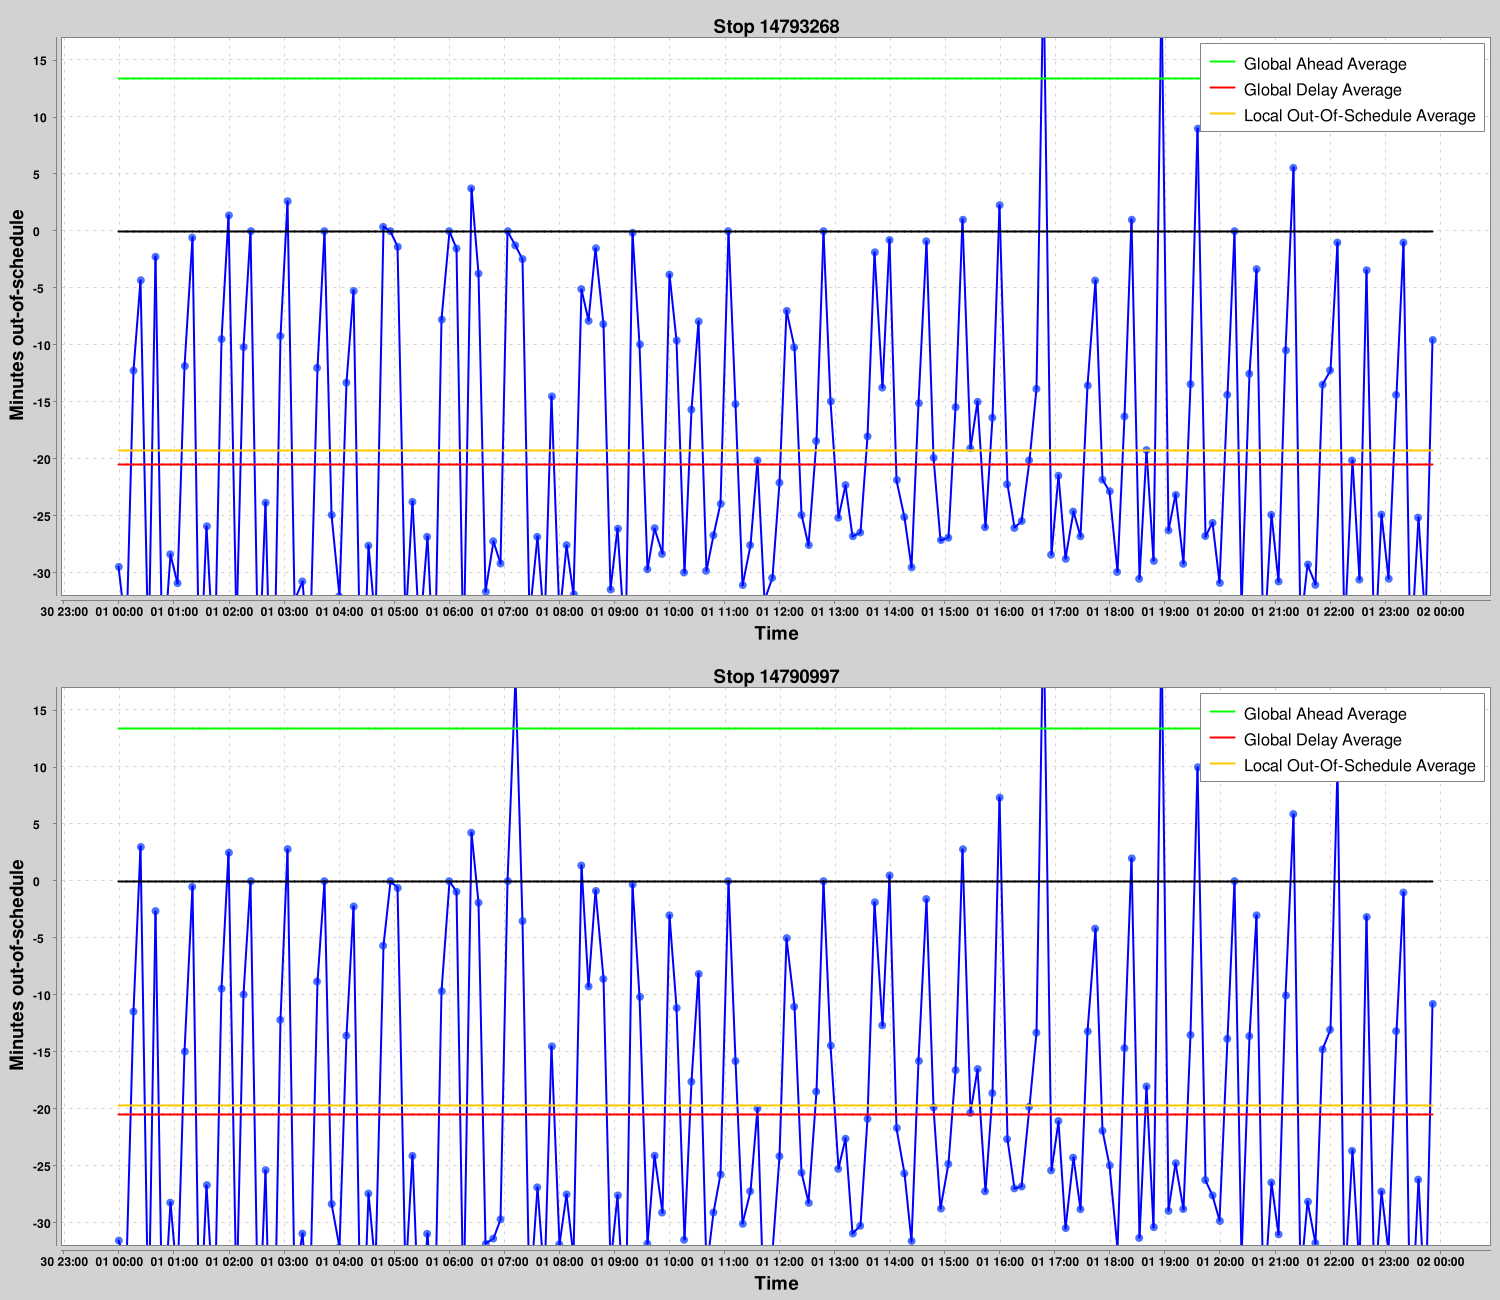
\includegraphics[width=\textwidth]{imagem/cap5/stops2.png}
        \source{The authors}
        \label{img:5:stops}
\end{figure}

For instance, using stop $\#14788408$, each blue dot in Figure \ref{img:5:stops2} denotes the average
minutes out-of-schedule for this stop in an instant in time. So, around 1:15 A.M., all the buses heading to this stop had an average
of 2 minutes ahead of schedule, and around 21:50 A.M., all the buses heading to this stop had an average of 9 minutes delayed.
Since the green and the red constants are global averages, they are unreliable for analyzing the delays due to the {\em log-normal}
distribution, but the yellow gives a more reliable insight to create a time-window interval, so for 
this stop, on average, the buses are delayed 3 minutes.


The stops $\#14793268$ and $\#14790997$ are the first and third most delayed in the PTN, respectively.
These stops are 462 meters from each other on the same avenue, \textit{Avenida Pedro II}, and share 2,590 common trips, so they are spatially related. Furthermore, they also have a temporal relationship, and 
Figure \ref{img:5:stops} works similarly to Figure \ref{img:5:stops2} and shows these stops on weekdays. Observing Figure \ref{img:5:stops}, the similarities of
delay distribution in these stops demonstrate the temporal relationship because 
both stops have similar frequencies of all statuses simultaneously: on time, ahead of schedule, and delayed. For instance, the early morning period from 4:00 A.M. to 7 A.M. is
practically equal with periods of intense delays, while the afternoon period starting at 5:00 P.M. reveals for both stops trips ahead of schedule. Also, these stops have a close \textit{Local Out-Of-Schedule Average}, which is $19.29$ minutes for $\#14793268$ and $19.68$ for minutes $\#14790997$, both are delays.



\section{Comparison Between Generated and Real Data}
The analysis shown in the two previous sections was only possible because Belo Horizonte's GTFS defines the expected time for all
bus stops on every trip. Belo Horizonte's GTFS provides this data despite not being required fields. 
As discussed in the previous Chapter, the \textit{Trip Expected Time Generator} generates the expected times when missing. In this section, we executed this component with Belo Horizonte's data and compared the expected times generated
with those defined at the GTFS. Table \ref{tab:delay2} displays the same data presented in Table \ref{tab:delay1}
but increasing it with the generated expected times.

\begin{table}[h]
\centering
\caption{Delays detailed in whole PTN scale with generated expected times}
\begin{tabular}{|c|c|c|r|r|}
\hline
\multicolumn{3}{|c|}{} &   GTFS  &  Generated  \\
\hline
 \multirow{5}{*}{\textbf{Weekday}} & \multicolumn{2}{|c|}{\textbf{Total trips matched}} &118,559 &  118,559 \\\cline{2-5}
 & \multicolumn{2}{|c|}{\textbf{Trips entirely out of schedule}} &60,244  & 57,843 \\\cline{2-5}
 & \multicolumn{2}{|c|}{\textbf{Trips with departure or arrival on time}} &39,403 & 39,526  \\\cline{2-5}
 & \multicolumn{2}{|c|}{\textbf{Trips with departure and arrival on time}} &324 & 393\\\cline{2-5}
 & \multicolumn{2}{|c|}{\textbf{Trips entirely on time}} &1&0 \\
\hline
 \multirow{5}{*}{\textbf{Saturday}} & \multicolumn{2}{|c|}{\textbf{Total trips matched}} &22,796 &  22,796\\\cline{2-5}
 & \multicolumn{2}{|c|}{\textbf{Trips entirely out of schedule}} & 10,899  & 10,497 \\\cline{2-5}
 & \multicolumn{2}{|c|}{\textbf{Trips with departure or arrival on time}} &8,731 & 8,723  \\\cline{2-5}
 & \multicolumn{2}{|c|}{\textbf{Trips with departure and arrival on time}} &95 & 130 \\\cline{2-5}
 & \multicolumn{2}{|c|}{\textbf{Trips entirely on time}} &2&0 \\
\hline
 \multirow{5}{*}{\textbf{Sunday}} & \multicolumn{2}{|c|}{\textbf{Total trips matched}} &15,273 &  15,273\\\cline{2-5}
 & \multicolumn{2}{|c|}{\textbf{Trips entirely out of schedule}} & 7,148  & 6,733 \\\cline{2-5}
 & \multicolumn{2}{|c|}{\textbf{Trips with departure or arrival on time}} &5,988 & 6,022  \\\cline{2-5}
 & \multicolumn{2}{|c|}{\textbf{Trips with departure and arrival on time}} &56 & 73 \\\cline{2-5}
 & \multicolumn{2}{|c|}{\textbf{Trips entirely on time}} &1&0 \\
\hline
\end{tabular}
\source{The authors}
\label{tab:delay2}
\end{table}

Table \ref{tab:delay2} shows that our generated data has some similarities and differences to the provided data and
using the generated data, Weekdays, Saturdays, and Sundays have fewer trips entirely out of schedule, $3.99$\%, $3.69$\%, and
$5.81$\%, respectively. 
On the one hand, this decrease points to a redistribution of the status $ON\_TIME$ throughout the network. %because the gross number of this status has decreased, as Figure \ref{img:5:pie} shows
On the other hand, this redistribution affected the four trips entirely on time, which are missing. 
Another point is that for all cases, except one, the generated schedule has
increased the number of trips with departure and/or arrival on time, and this occurs due to the minor alterations to the 
$departure\_time$ field caused by the \textit{DefaultTripExpectedTimeGenerator}, which were used. 
Saturday's trips with departure or arrival on time is the scenario that the generated data was outperformed by $0.09$\%,
virtually, they performed equally. 

Furthermore, Table \ref{tab:delaydistribution} presents statuses throughout the bus stops for the GTFS and the expected times
generated. For both scenarios, the $DELAYED$ status is predominant in the network, followed by the $AHEAD\_OF\_SCHEDULE$ and
$ON\_TIME$, respectively. Also, Table \ref{tab:delaydistribution} shows an expressively increase in $AHEAD\_OF\_SCHEDULE$
, and an expressively decrease for $DELAYED$, and a minor decrease for $ON\_TIME$ when using the generated data. 
Despite the $DELAYED$ status having the most occurrences, it does not denote that the PTN is completely stopped or delayed due to the
{\em log-normal} distribution of this status, as discussed in the previous Section.

\begin{table}[h!]
\centering
\caption{Statuses Distribution for Bus Stops}
\begin{tabular}{|c|c|c|r|r|}
\hline
\multicolumn{3}{|c|}{} &   GTFS  &  Generated  \\
\hline
 \multirow{3}{*}{Weekday} & \multicolumn{2}{|c|}{$ON\_TIME$} & $3.3\%$ & $3.2\%$ \\\cline{2-5}
 & \multicolumn{2}{|c|}{$AHEAD\_OF\_SCHEDULE$} & $6.9\%$ & $17.8\%$ \\\cline{2-5}
 & \multicolumn{2}{|c|}{$DELAYED$} &$89.8\%$ & $79.0\%$  \\
\hline
 \multirow{3}{*}{Saturday} & \multicolumn{2}{|c|}{$ON\_TIME$} & $3.9\%$ & $3.5\%$ \\\cline{2-5}
 & \multicolumn{2}{|c|}{$AHEAD\_OF\_SCHEDULE$} & $6.5\%$ & $18.4\%$ \\\cline{2-5}
 & \multicolumn{2}{|c|}{$DELAYED$} &$89.6\%$ & $78.1\%$  \\
\hline
 \multirow{3}{*}{Sunday} & \multicolumn{2}{|c|}{$ON\_TIME$} & $4.4\%$ & $3.9\%$ \\\cline{2-5}
 & \multicolumn{2}{|c|}{$AHEAD\_OF\_SCHEDULE$} & $5.4\%$ & $18.5\%$ \\\cline{2-5}
 & \multicolumn{2}{|c|}{$DELAYED$} &$90.2\%$ & $77.6\%$  \\
\hline
\end{tabular}
\source{The authors}
\label{tab:delaydistribution}
\end{table}


Finally, Figure \ref{img:5:stops_generated} presents the same couple of stops from Figure \ref{img:5:stops} but using the
generated expected times. With the generated data, the \textit{Global Ahead Average} and the \textit{Global Delay Average}
are $38.57$ and $24.75$ minutes, respectively. This denotes that the interval of out-of-schedule is wider using the generated data. Still, on the other side, the \textit{Local Out-Of-Schedule Average} show smaller delays for the stops $\#14793268$ and $\#14790997$, $15.54$ and $14.68$ minutes respectively. This data points out that despite increasing the global averages, our 
approach decreased the average delay in two of the most delayed stops from the PTN by $3.75$ and $5$ minutes, respectively.

\begin{figure}[h]
     \centering
        \caption{Minutes out of schedule of a couple of bus stops distributed throughout the day using generated data}
        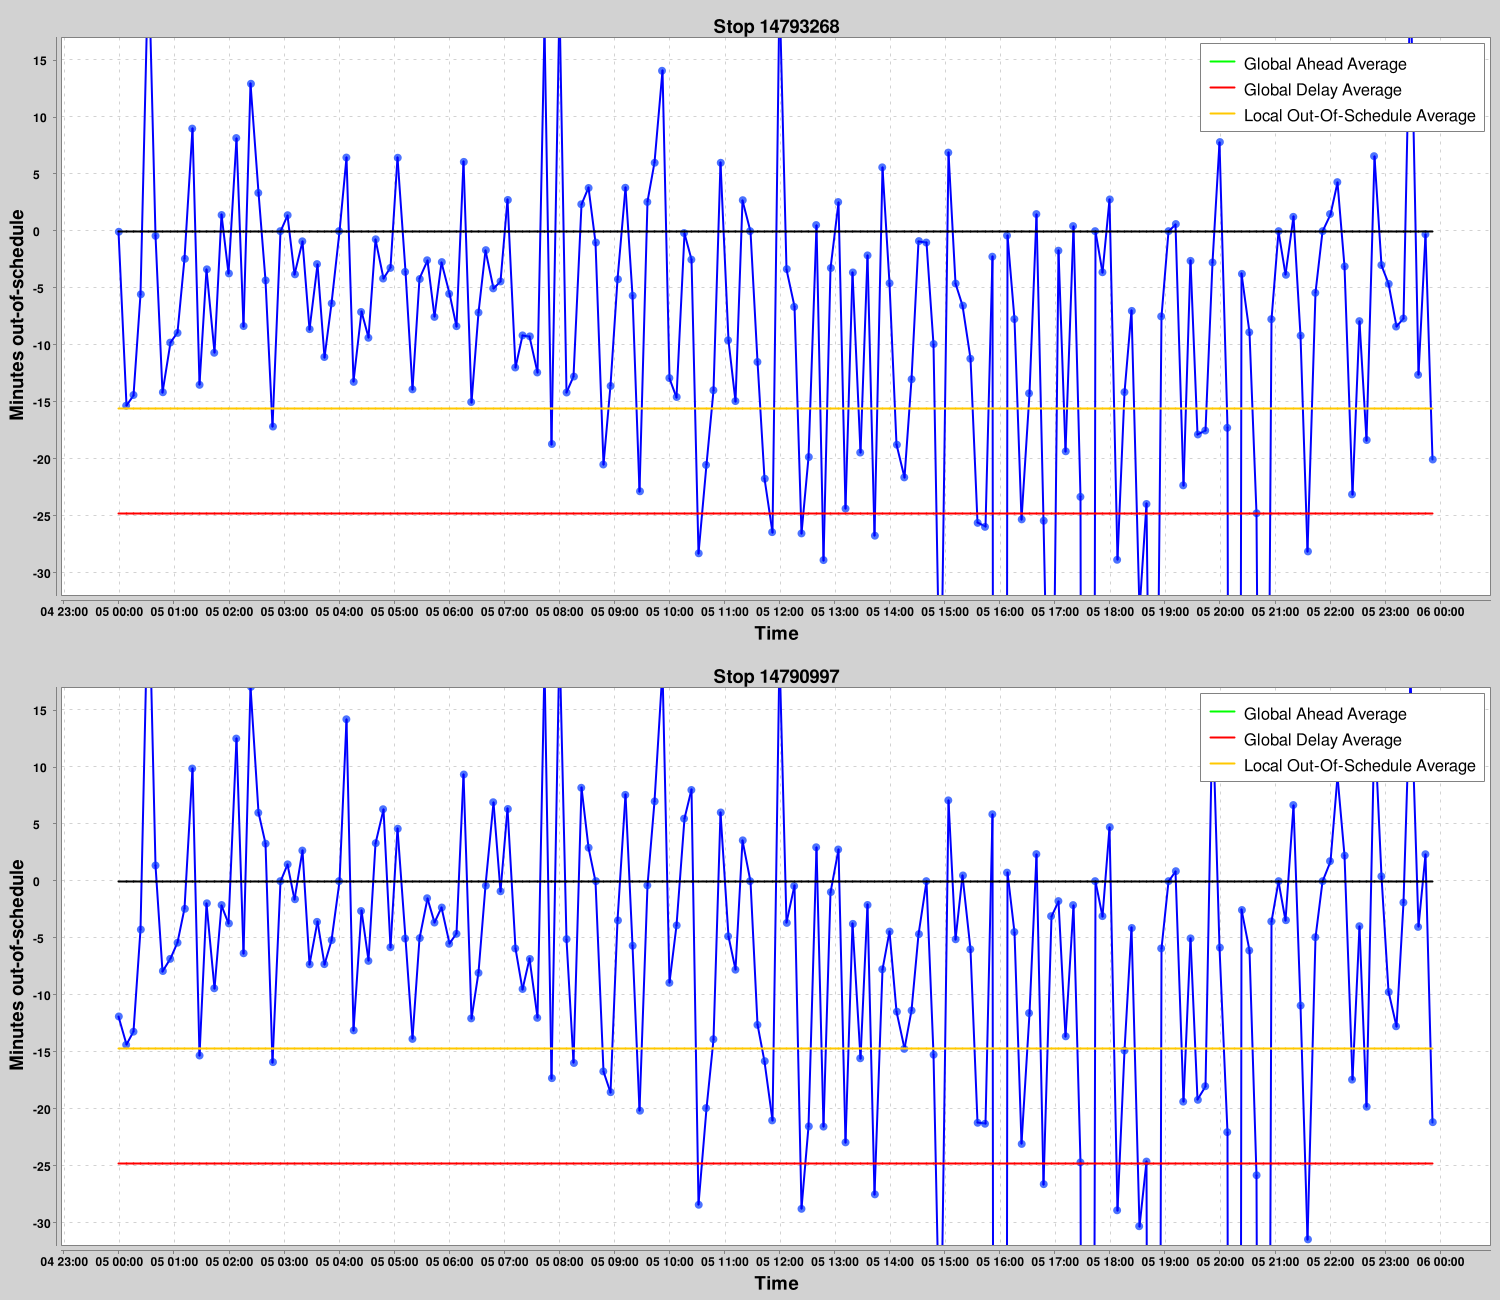
\includegraphics[width=\textwidth]{imagem/cap5/stops2_generated.png}
        \source{The authors}
        \label{img:5:stops_generated}
\end{figure}

\section{Limitations}
We acknowledge some limitations, mainly due to the desynchronization
between the datasets. For instance, the {\em Real-Time Data Collector} is the most fragile component due
to the third-party real-time traffic API interface, which creates minor issues,
such as providing some unwanted trips. And some significant problems, such as 
the impossibility of linking an entry to a trip. Also, the crucial point is that the size and quality of 
the real-time data heavily depend on the API refresh timeout, in which smaller
timeouts translate to more bus positioning, which improves the accuracy of generating
artificial entries.

We acknowledge the lack of methods to make a comparison, we discussed about all the others similar scenarios found in literature in Chapter 3.
Also, \textit{PondiônsTracker} fails to capture unexpected events that affect the traffic such as concerts because these events {\em may} not be represented by the GTFS. 
Thus, two routes are scheduled in the GTFS, but they did not have any entry reported by the real-time API, which are 
the two following routes:
\begin{enumerate*}
    \item \textit{720 - Circular Saúde MG20} missed $175$ trips;
    \item \textit{912 - Conjunto Taquaril/Praça Che Guevara} missed $210$ trips.
\end{enumerate*}

